\documentclass{amsart}

\newif\ifcref\creftrue
%\usepackage{overrightarrow}
\makeatletter
\newcommand\reldoublebar{\mathrel{\smash=}}
\newcommand{\Rightarrowfill@@}[1]{%
\m@th \setboxz@h {$#1\reldoublebar $}\ht \z@ \z@ 
$#1\copy \z@ 
\mkern -6mu\cleaders \hbox {$#1\mkern -2mu\box \z@ \mkern -2mu$}\hfill 
\mkern -6mu
\mathord \Rightarrow $}
\newcommand{\Overrightarrow}{\mathpalette{\overarrow@\Rightarrowfill@@}}
\makeatother

\input{decls}
\usepackage{ifmtarg,tikz,mathpartir}
\tikzset{lab/.style={auto,font=\scriptsize}} % arrow labels
\usetikzlibrary{arrows}
\usetikzlibrary{shapes.geometric,shapes.arrows}
\newenvironment{tikzc}[1][]{\begin{center}\begin{tikzpicture}[#1]}{\end{tikzpicture}\end{center}}
\tikzset{>=stealth}
\tikzset{ed/.style={auto,inner sep=0pt,font=\scriptsize}} %edges
\tikzset{arr/.style={draw,isosceles triangle,inner sep=2pt}} %arrows

\newcommand{\C}{\cC}
\newcommand{\D}{\cD}
\renewcommand{\Chat}{\ensuremath{\widehat{\C}}\xspace}
\newcommand{\Chats}{\ensuremath{\Chat_{\Sigma}}\xspace}
\newcommand{\thhat}{\ensuremath{\widehat{\theta}}\xspace}
\newcommand{\thchk}{\ensuremath{\widecheck{\theta}}\xspace}
\newcommand{\E}{\cE}
\newcommand{\F}{\cF}
\newcommand{\G}{\cG}
\newcommand{\V}{\cV}
\newcommand{\W}{\cW}
\newcommand{\K}{\bbK}

\newcommand{\Hkl}[2]{\mathbb{H}\text{-}\mathsf{Kl}(#1,#2)}
\newcommand{\Hcokl}[2]{\mathbb{H}\text{-}\mathsf{coKl}(#1,#2)}
\newcommand{\Hbikl}[2]{\mathbb{H}\text{-}\mathsf{biKl}(#1,#2)}

\newcommand{\one}{\lone}
\newcommand{\bone}{\mathbf{1}}

\autodefs{\cMod\dCat\bCat\dSpan\dMod\bSet\bGraph\dMod\cMod}
\let\Mod\dMod
\let\mod\cMod
\def\modk{\mod_\K}
\def\mor#1{\hom_{#1}}

\def\cart{\chi}
\def\opcart{\chi}
\def\emptyvec#1{()_{#1}}
\def\unit#1{\hom_{#1}}
\def\bigcomp{\textstyle\bigodot\!}

\newcommand{\blank}{\mathord{\hspace{1pt}\text{--}\hspace{1pt}}}
\newcommand{\uniq}{\mathord{!}}
\renewcommand{\o}{^{\circ}}
\newcommand{\p}{^{+}}
\newcommand{\m}{^{-}}
\newcommand{\e}[1][]{^{\varepsilon_{#1}}}
\newcommand{\epbar}{^{\varepsilon^*}}
\renewcommand{\ph}[1][]{^{\varphi_{#1}}}
\newcommand{\phe}[2]{^{\varphi_{#1}\varepsilon_{#2}}}
% \let\vec\overrightarrow
% \let\Vec\Overrightarrow
%\renewcommand{\Vec}[1]{\overset{\Rightarrow}{#1}}

\def\types{\;\vdash\;} % turnstile
\let\mto\vdash    % As a hom operator on modules
\def\mhom#1#2{\left( #1 \vphantom{\big|}\mto #2 \right)}
\def\mhomc#1#2#3{\left( #1 \mid #2 \vphantom{\big|}\mto #3 \right)}
\def\cb{\;\mid\;} % context break
\newcommand\combine{,}
\newcommand\combineU{\sqcup}
\def\flip#1{#1^*} % reverse the variances of all variables
\newcommand{\unif}[4]{#1\doteq #2\,\mathsf{ via }\,#3\cb #4}
\newcommand{\coend}{\begingroup\textstyle\int\endgroup}
\newcommand{\tend}{\begingroup\textstyle\int\endgroup}
\newcommand{\subst}[3]{{#1}[#2 \mapsfrom #3]}
\newcommand{\ev}{\mathsf{ev}}

\title{Multivariable formal category theory}
\author{Patrick Schultz and Michael Shulman}
\begin{document}
\maketitle

\setcounter{tocdepth}{1}
\tableofcontents

\section{Introduction}
\label{sec:intro}

We propose a categorical structure designed for doing ``multivariable formal category theory'', including particularly contravariant functors and extraordinary natural transformations, and hence the abstract study of monoidal objects, enriched objects, multivariable adjunctions, closed objects, rigid objects, and so on.
This is analogous to how proarrow equipments~\cite{wood:proarrows-i} and Yoneda structures~\cite{street-walters:yoneda} provide abstract contexts for doing one-variable formal category theory.
By analogy with the word ``equipment'', we call our structure a \textbf{kit}.

There does already exist one structure in which one can do multivariable formal category theory.
As observed by Day and Street~\cite{ds:monbi-hopfagbd}, the opposite of a category is its dual in the monoidal bicategory of profunctors, making the latter ``compact closed'' (also called ``rigid'' or ``autonomous''); and inside a compact closed bicategory one can define structures of multivariable category theory.
Of course, the bicategory of profunctors does not quite know which profunctors are representable by functors (the left adjoint profunctors are ``representable up to Cauchy completion''), but this can be remedied by enhancing it to a ``compact closed proarrow equipment''.

The differences between a kit and a compact closed equipment, and hence the reasons for defining the former, are:
\begin{enumerate}
\item Compact closed equipments have not actually been defined yet either, and it's not necessarily \emph{a priori} obvious how much coherence should be required between the ``functor arrows'' and the compact closed structure.
  (As observed in~\cite{shulman:contravariance}, even for just the one-variable ``opposite category'' operation there are nontrivial coherence questions.)
  The definition of a kit is ``more obviously complete''.
  Below, we will actually also define compact closed equipments and prove that any such gives rise to a kit, justifying that definition.
\item A kit is ``fully virtual'' in the sense of~\cite{cs:multicats}; that is, all of its structure is multicategorical.
  This means that rather than including \emph{operations} such as profunctor composition, monoidal product, and dualization, a kit includes a basic notion of ``morphism out of such things'', in the same way that a multicategory has no actual monoidal product but includes a basic notion of ``multivariable morphism'' that ``would be a morphism out of a monoidal product if it existed''.
  This allows these operations, when they exist, to be characterized by universal properties, eliminating the question of what coherence axioms have to be imposed upon them as structure.
  It also allows us to describe examples where such operations do \emph{not} exist.
  For instance, categories enriched over any monoidal category \bV form a kit, whether or not \bV has any limits or colimits; indeed \bV could be only a multicategory itself.
\item Because of virtuality, it is much simpler to define sub-kits and quotient kits.
  In particular, this allows us to construct ``homotopy kits'' by first restricting to a subclass of well-behaved objects, then quotienting by a homotopy relation.
  This gives one approach to formal higher category theory using only 2-categorical machinery.
  %% The quasicategorical case is probably easiest to do by going via a compact ordinary equipment, adding opposites to the Riehl-Verity construction.  But this approach probably works for 2Cat-Gray, and might for higher ones using the lax monoidal structures.
\item A kit eliminates the ``two-sided bias'' of a bicategory or an equipment.
  Two-sidedness is appropriate and necessary for one-variable category theory, since in examples such as categories enriched in a non-symmetric monoidal category (or in a bicategory) the only ``modules'' that can be defined are covariant in exactly one variable and contravariant in exactly one other variable.
  But for multivariable category theory, where a module can naturally be covariant in many variables and contravariant in many other variables, it feels artificial to divide these variables into a ``domain'' and a ``codomain'', forcing us to pass back and forth across dualization equivalences when we want to compare a profunctor $A \hto B\times C$ with a profunctor $C\op\times A \hto B$, while intuitively (and in most examples) there is really only one notion involved, namely a functor $B\op \times C\op \times A \to \bSet$.
  (Lest the reader worry about generality, categories enriched in a non-symmetric monoidal category do still form a kit; it just happens to be a kit all of whose modules depend on one covariant variable and one contravariant one.
  More generally, any equipment can be regarded directly as a kit in this way.)
\item Finally, a kit furnishes a more natural semantics for the ``directed type theory'' of~\cite{lnss:dirtt}, because its classes of objects and morphisms correspond directly to the judgments of the latter.
  In particular, a kit admits a very familiar set-like ``internal-language'' in which to reason about its objects, analogous to the ``abstract index notation'' of tensor calculus.
  We will introduce this language informally here; for details see~\cite{lnss:dirtt}.
\end{enumerate}

\part{Multivariable formal category theory}
\label{part:mfct}

In this part we will describe the structure of a kit informally, and consider a number of examples of how to use that structure to formulate category-theoretic arguments abstractly.
The formal definition of a kit is rather technically involved and occupies \cref{part:def}; but this part is intended to demonstrate that for nearly all practical applications it is not necessary to know the details of the formal definition, only to have faith that it exists and behaves as one would expect.

\section{The structure of a kit}
\label{sec:structure}

A kit is composed of four sorts of things, which we discuss in turn.

\subsection{Cats}

There is a class of objects, which we call \textbf{cats}, since they play the role of categories.

\subsection{Functors}

We generally call the morphisms between cats \textbf{functors}.
This is in line with the fact that the morphisms between many different kinds of generalized categories --- enriched categories, indexed categories, bicategories, $\infty$-categories, etc. --- are frequently called just ``functors'' without qualification.

The functors in a kit are functors of many variables, some covariant and some contravariant.
More precisely, the domain of a functor is a finite list of cats, some of which are annotated with the formal symbol $(-)\o$ to indicate contravariance.
(This does not yet represent an operation of ``oppositization'' on cats; it is just a formal marker for contravariance.
Similarly, we do not in general assume a ``tensor product'' of cats; as we will see later, these operations can be characterized by universal properties in terms of the multivariable functors.)
The codomain of a functor, by contrast, is a single cat; thus we might have for instance $f:(A,B\o,C) \to D$.
If the list contains only one cat, we generally omit the parentheses, writing $f:A\to B$.

Functors can be composed in a ``multicategorical'' way that keeps track of variance.
For instance, if in addition to $f:(A,B\o,C) \to D$ we have $g:X \to A$ and $h:(Y\o,Z)\to B$ and $k:()\to C$ (yes, lists can have length zero), then there is a composite $f\circ (g,h,k) : (X,Y,Z\o)\to D$.
Finally, like in a symmetric multicategory, we have symmetric group actions on the domains of functors, so that from $f:(A,B\o,C) \to D$ we can obtain a functor $(B\o,C,A)\to D$ and so on.

In particular, we have a category of cats and unary functors, which we denote $\K_1$.
Later on we will enhance this to a 2-category.

\subsection{Modules}

Now we have a second class of objects, which we call \textbf{modules}; these represent presheaves, profunctors, and more general ``functors into the base of enrichment''.
Each module is indexed by a finite list of cats with variance (the same sort of list that appears as the domain of a functor).
We write $\modk(A,B\o,C)$ for the category (see below) of modules indexed by a list $(A,B\o,C)$.
Modules can be restricted along functors; thus if $M\in \modk(A,B\o,C)$, and $g,h,k$ are as above, we have $(g,h,k)^*M \in \modk(X,Y,Z\o)$.
This restriction is strictly functorial with respect to functor composition (one could consider generalizations of a kit where it is only weakly functorial, but in most examples it is strict, and in other cases it can be modified to become so).

The symmetric groups also act on modules; thus if $M\in \modk(A,B\o,C)$ we have a module $\sigma^*M\in \modk(B\o,C,A)$ and so on.
As with restriction, we assume for simplicity that this action is strict.
Formally, the symmetric group action is combined with the restriction along functors, by representing the collection of modules as a functor defined on a category whose objects are lists of cats with variance and whose morphisms are lists of functors together with a permutation of their combined input.

\subsection{Module morphisms}

Finally we have module morphisms; this is where all the subtlety and difficulty lies.
The simplest sort of morphism between modules is an ``ordinary'' one between modules indexed by the same list of cats.
These form the morphisms of the categories such as $\modk(A,B\o,C)$, and restriction along functors is of course functorial on these categories.

The next simplest sort of module morphism is a ``multivariable'' one that represents a potential ``tensor product of modules'' multicategorically, similarly to how the multivariable functors represent a potential tensor product of categories.
Since our intended models include categories enriched over a non-cartesian base, the individual categories such as $\modk(A,B\o,C)$ are not necessarily monoidal (that is, we can't necessarily take a pointwise tensor product of presheaves), but we can expect ``external'' products such as $\modk(A) \times \modk(B) \to \modk(A,B)$.
Thus, representing these multicategorically we have multivariable module morphisms such as $(M_1,M_2,\dots,M_n) \to N$, where $M_i\in \modk(\Psi_i)$ and $N\in\modk(\Psi_1,\Psi_2,\cdots,\Psi_n)$, where $(\Psi_1,\Psi_2,\cdots,\Psi_n)$ indicates the concatenated list of cats with variance.
As with functors, the symmetric groups act on the domains of such morphisms.

However, in order to really do multivariable category theory, we also need ``extra\-ordinary'' natural transformations as in~\cite{ek:gen-funct-calc}.
For instance, given $M\in\modk(A,A\o,B)$ and $N\in \modk(C,C\o,B)$ we want to speak about a transformation $\alpha:M\to N$ that is ordinary natural in $B$ and extraordinary natural in $A$ and $C$ on either side.
In plain set-based category theory this means we have components $\alpha_{a,b,c}:M(a,a,b) \to N(c,c,b)$ such that the following naturality squares commute for all $f:a_1\to a_2$, $g:b_1\to b_2$, $h:c_1\to c_2$, and $a,b,c$:
\begin{mathpar}
  \xymatrix{ M(a,a,b_1) \ar[d]_{M(1,1,g)} \ar[r]^{\alpha} &
    N(c,c,b_1) \ar[d]^{N(1,1,g)}\\
    M(a,a,b_2) \ar[r]_{\alpha} & N(c,c,b_2)}\and
  \xymatrix{ M(a_1,a_2,b) \ar[d]_{M(1,f,1)} \ar[r]^{M(f,1,1)} &
    M(a_2,a_2,b) \ar[d]^{\alpha}\\
    M(a_1,a_1,b) \ar[r]_{\alpha} & N(c,c,b)}\and
  \xymatrix{ M(a,a,b) \ar[d]_{\alpha} \ar[r]^{\alpha} &
    N(c_2,c_2,b) \ar[d]^{N(1,h,1)}\\
    N(c_1,c_1,b) \ar[r]_{N(h,1,1)} & N(c_2,c_1,b)}
\end{mathpar}
Thus, a kit includes a set of ``extraordinary'' module morphisms from $M$ to $N$ whenever $M\in \modk(\Psi_1, \Psi_1\o, \Psi_2)$ and $N\in\modk(\Psi_3, \Psi_3\o, \Psi_2)$.
Here the $\Psi_i$ are lists of cats with variance, and $\Psi\o$ denotes reversal of all the variances in $\Psi$.
Of course, in general the cats we want to match up extraordinarily may not appear in exactly this order (e.g.\ we could have $M\in \modk(A,B,A\o)$ and $N\in \modk(B,C\o,C)$), but we can first act on the modules by a permutation.

The extraordinary morphisms, like the ordinary ones that form the arrows of the categories $\modk(\Psi)$, can be restricted along functors, in a functorial way.
Specifically, given $M\in \modk(\Psi_1, \Psi_1\o,\Psi_2)$ and $N\in\modk(\Psi_3, \Psi_3\o,\Psi_2)$ as above, determining a type of extraordinary module morphism from $M$ to $N$, then such module morphisms can be restricted along any lists of functors $f_i:\Psi_i' \to \Psi_i$ (for $i=1,2,3$).
Here $f_i$ consists of a functor with codomain $A$ for each cat $A$ in $\Psi_i$, and $\Psi_i'$ is the concatenated list of the domains of these functors, with the variance of each $A$ in $\Psi_i$ applied to the domain of the corresponding functor.
Thus for instance if $g:(A,B\o) \to C$ and $h:D\to E$, we would have $(g,h):(A,B\o,D\o) \to (C,E\o)$.
Note that just as the domain and codomain of an ordinary module morphism have to be restricted along the same functor (since restriction defines functors $\modk(\Psi) \to \modk(\Psi')$), the two occurrences of a cat in the domain or codomain in an extraordinary morphism also have to be restricted along the same functor.

Finally, we can have multivariable extraordinary morphisms as well, where the domain is a list of modules rather than a single one.
In this case we almost always want to permute the lists of cats appearing in the domain rather than simply concatenating them, so technically we have to incorporate a notion of permutation action on a list; in a moment we will introduce a more convenient notation for this.

The real complication comes when defining how extraordinary morphisms can be \emph{composed}.
The rules for how to compose extraordinary natural transformations were given in~\cite{ek:gen-funct-calc}, but it seems to be quite involved to use these rules to define an abstract structure in a categorically respectable way.
In \cref{sec:composing} we will describe the rules informally; but first we digress to introduce a better notation for extraordinary morphisms.


\section{Abstract variable notation}
\label{sec:tt}

It turns out to be quite convenient to use a different notation for modules and their morphisms.
Rather than writing
\[ M \in \modk(A,B\o,C) \]
we allow ourselves to think of $M$ as a functor that takes ``values'' on ``variables'' belonging to $A,B,C$, and write
\[ \ctx{a:A,b:B\o,c:C} \types M(a,b,c) \in\modk. \]
Note that the cats in a kit are still just abstract objects; we are not asserting that they have ``elements'' in any sense.
These ``variables'' are purely schematic.
This is very much like the ``abstract index notation'' of tensor calculus that allows us to write $T^{a b}_{c}$ for an element of a tensor space $V \otimes V\otimes V^*$ without needing to actually pick a basis of $V$ to make $a,b,c$ into actual numerical indices of components.

One reason this ``abstract variable notation'' is useful is when restricting modules along functors.
In the previous example with $M$ as above and
\begin{mathpar}
  g:X \to A \and h:(Y\o,Z)\to B \and k:()\to C
\end{mathpar}
instead of $(g,h,k)^*M \in \modk(X,Y,Z\o)$ we can write
\[ \ctx{x:X,y:Y,z:Z\o}\types M(g(x),h(y,z),k)\in\modk \]
This indicates much more clearly how the functors $g,h,k$ match up with the dependence of $M$ on $A,B\o,C$ and how the resulting dependence on $X,Y,Z\o$ feeds into $g,h,k$.
The strict functoriality of restriction with respect to functor composition means that this notation behaves as we expect on such composites; for instance, if we have
\begin{mathpar}
  \ctx{c:C}\types M(c)\in\modk \and g:B\to C \and f:A\to B
\end{mathpar}
then the three restrictions $g^*M$, $f^*g^*M$, and $(g\circ f)^*M$ are represented in this notation as
\begin{mathpar}
  \ctx{b:B}\types M(g(b)) \in\modk\\
  \ctx{a:A}\types M(g(f(a))) \in\modk\and
  \ctx{a:A}\types M((g\circ f)(a)) \in\modk
\end{mathpar}
where the second and third are, as we expect, equal.

The second place that abstract variable notation is useful is when describing module morphisms, and especially extraordinary ones.
We said above that extraordinary module morphisms go from $M$ to $N$ whenever $M\in \modk(\Psi_1, \Psi_1\o, \Psi_2)$ and $N\in\modk (\Psi_3, \Psi_3\o, \Psi_2)$.
We also mentioned that we generally have to apply a permutation in order to put the lists of cats in exactly this form, such as if $M\in \modk(A,B,A\o)$ and $N\in \modk(B,C,C\o)$.
In practice, instead of actually acting on $M$ and $N$ by symmetric groups, it is easier to just indicate how the cats should be matched up.
We can do this with abstract variables as follows:
\[ \ctx{a:A,b:B,c:C} \cb M(a,b,a) \types N(b,c,c) \]
Note that every variable appears exactly twice to the right of the vertical bar, once covariantly and once contravariantly (where occurrences to the left of the turnstile $\vdash$ are counted with opposite variance).

This notation is especially valuable when the same cat appears multiple times.
For instance, if $M\in\modk(A,A\o,A)$ and $N\in\modk(A)$, then there are two kinds of extraordinary morphisms from $M$ to $N$, which are represented in this notation as
\begin{mathpar}
  \ctx{x:A,y:A} \cb M(x,x,y)\types N(y)\\
  \ctx{x:A,y:A} \cb M(x,y,y)\types N(x)
\end{mathpar}
It is also especially useful when talking about multivariable extraordinary morphisms.
For instance, we could have
\[ \ctx{a:A,b:B,c:C,d:D} \cb M_1(a,b), M_2(b,c) \types N(a,d,c,d) \]
but here there is no way to act on $M_1$ and $M_2$ by symmetric groups separately to put the $B,B\o$ in front.
Formally, this means that when describing multivariable extraordinary morphisms we have to incorporate a permutation in the definition; but with abstract variable notation we don't need to think about that.

Finally, if the cats that the variables correspond to are obvious from context, we can omit their declarations, obtaining a more concise notation $M(a,b,a) \mto N(b,c,c)$ for a set of extraordinary module morphisms.
Thus, if we want to give a name to a particular such morphism we can write
\[ \phi \in \mhom{M(a,b,a)}{N(b,c,c)} \]

It is worth emphasizing one difference between the use of abstract variables for restriction and for extraordinary morphisms.
In the case of restriction, we write $M(f(a),g(b))$ to denote the \emph{actual module} $(f,g)^*M$ obtained by restricting $M$ along $f$ and $g$.
However, in the case of extraordinary morphisms, it is probably better not to think of the notation $M(a,a)$ as actually denoting any module distinct from $M$;\footnote{In the formal definition to be presented in \cref{part:def}, it is possible to think of $M(a,a)$ as an object of ``$S\E$'', but this is arguably just a technical device.} in particular it is not obtained by restriction of $M$ along any sort of ``diagonal'' (which need not exist in an arbitrary kit).
We will also combine these notations, writing for instance $M(f(a),g(a),h(b))\mto N(k(b))$; in this case it is better to think of the restrictions as happening first (obtaining modules such as $M(f(a_1),g(a_2),h(b))$), followed by the pairing of variables to determine a type of extraordinary morphism.

So far we have described our ``abstract variable notation'' somewhat informally.
When doing formal category theory, this informal understanding is generally sufficient.
However, the notation can in fact be made much more precise, by defining a type theory to serve as the ``internal language'' of a kit; see~\cite{lnss:dirtt}.

\section{Composing extraordinary morphisms}
\label{sec:composing}

The simplest sort of composition for extraordinary morphisms is composition with ordinary ones on either side.
For instance, a morphism $\phi\in \mhom{M(a,b,a)}{N(b,c,c)}$ can be composed with an ordinary map $\psi:N\to N'$ in $\modk(B,C,C\o)$ to obtain a morphism $\psi\phi\in \mhom{M(a,b,a)}{N'(b,c,c)}$
In examples it is easy to see how to do this: just compose the components
\[ M(a,b,a) \xto{\phi_{a,b,c}} N(b,c,c) \xto{\psi_{b,c,c}} N'(b,c,c) \]
and check that the naturality relations (both ordinary and extraordinary) are preserved.
(Note that the components $\psi_{b,c_1,c_2}$ with $c_1\neq c_2$ do not appear in the definition, but they do appear in the proof of extraordinary naturality.)
Formally, we can say that each set of extraordinary morphisms admits an action on both sides by the categories $\modk(\Psi)$ (that is, it is a profunctor).

More interesting sorts of composition involve two extraordinary transformations, as explained in~\cite{ek:gen-funct-calc}.
The most basic composite of this sort involves two morphisms
\begin{mathpar}
  \phi\in \mhom{M(x)}{N(x,y,y)} \and \psi\in\mhom{N(z,z,w)}{P(w)}.
\end{mathpar}
with $x,y,z,w$ all associated to the same cat $A$.
In examples, we can compose these by composing their components
\[ M(x) \xto{\phi_{x,x}} N(x,x,x) \xto{\psi_{x,x}} P(x) \]
and check that the result is an ordinary natural transformation $M\to P$.

Note that the identification of all three variables in $N$ is mandated in order to be able to write both $\phi$ and $\psi$, since $\phi$ requires the second and third variables to be the same while $\psi$ requires the first and second to be the same.
This then determines how the naturality of the composite matches up the variables of $M$ and $P$ (in this case, of course, they have only one variable each, but in general they might have many and this matching might be ambiguous).
This process of identifying variables can be represented by drawing a graph:
\begin{center}
  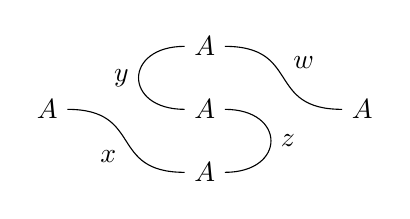
\begin{tikzpicture}[xscale=2,yscale=.8]
    \node (A1) at (0,0) {$A$};
    \node (A2a) at (1,1) {$A$};
    \node (A2b) at (1,0) {$A$};
    \node (A2c) at (1,-1) {$A$};
    \node (A3) at (2,0) {$A$};
    \draw (A1) to[out=0,in=180] node[auto,swap] {$x$} (A2c);
    \draw (A2a) to[out=0,in=180] node[auto] {$w$} (A3);
    \draw (A2a) to[out=180,in=180] node[auto,swap] {$y$} (A2b);
    \draw (A2b) to[out=0,in=0] node[auto] {$z$} (A2c);
  \end{tikzpicture}
\end{center}
or by solving a system of equations that ``unifies'' each arguments of the codomain $N(x,y,y)$ of $\phi$ with the corresponding argument of the domain $N(z,z,w)$ of $\psi$:
\begin{mathpar}
  x=z \and y=z \and y=w
\end{mathpar}

There are cases where this doesn't work; that is, pairs of extraordinary morphisms from $M$ to $N$ and from $N$ to $P$ that are ``non-composable'' despite having the same module $N$ in the middle.
For example, we might instead have
\begin{mathpar}
  \phi\in \mhom{M(x)}{N(x,y,y)} \and \xi\in\mhom{N(w,z,z)}{P(w)}.
\end{mathpar}
The problem here is that when ``composing components'' there is no way to decide what $y$ and $z$ should be: we can write down the composite
\[ M(x) \xto{\phi_{x,y,y}} N(x,y,y) \xto{\xi_{x,y,y}} P(x) \]
for any value of $y$, and there is no canonical choice (note that $x$ and $w$ might belong to an entirely different cat, so choosing $y=x$ is not an option).
Graphically, this problem is visible as the presence of a ``loop'':
\begin{center}
  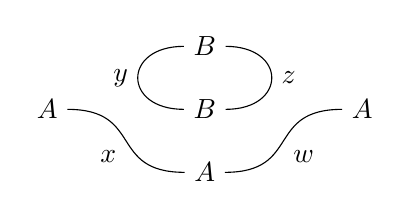
\begin{tikzpicture}[xscale=2,yscale=.8]
    \node (A1) at (0,0) {$A$};
    \node (A2a) at (1,1) {$B$};
    \node (A2b) at (1,0) {$B$};
    \node (A2c) at (1,-1) {$A$};
    \node (A3) at (2,0) {$A$};
    \draw (A1) to[out=0,in=180] node[auto,swap] {$x$} (A2c);
    \draw (A2c) to[out=0,in=180] node[auto,swap] {$w$} (A3);
    \draw (A2a) to[out=180,in=180] node[auto,swap] {$y$} (A2b);
    \draw (A2a) to[out=0,in=0] node[auto] {$z$} (A2b);
  \end{tikzpicture}
\end{center}
A more careful explanation of this condition, and a proof that it is the most general answer (for the classical case of enriched categories), can be found in~\cite{ek:gen-funct-calc}.

The technical work in the precise definition of a kit is to make precise \emph{all} the allowable composites of extraordinary morphisms, how they interact with restriction along functors, and in what sense these composites must be ``associative''.
However, in practical applications this generality is rarely needed, as most extraordinary morphisms only involve a few variables, and intuition from ordinary category theory is generally sufficient to give the right answer.
We intend to demonstrate this with some examples of doing ``formal category theory'' in a kit; but first we need to discuss some universal properties of cats and modules.

\section{Universal constructions}
\label{sec:univ}

Universal constructions in a kit are more complicated than those in an ordinary category, due to the interaction of the different kinds of morphisms.
Specifically, universal properties of cats generally have to be extended to say something about modules and module morphisms, while universal properties of modules have to include the extraordinary module morphisms somehow and also be stable under restriction along functors.

\subsection{Tensor products of cats and opposites}
\label{sec:tens-opp}

We begin with the simplest universal properties for cats: those that directly internalize the operations represented ``virtually'' by the multicategorical nature of functors.
For instance, a tensor product of cats $A,B$ should be a cat $A\otimes B$ with a functor $\chi:(A,B)\to A\otimes B$ through which any functor $(A,B)\to C$ factors uniquely.

However, this plain universal property, though it suffices to determine $A\otimes B$ uniquely up to isomorphism, is insufficient in several ways.
Firstly, as in the case of ordinary multicategories, it needs to apply to more general functors containing $(A,B)$ as only part of their domain.
Secondly, it needs to apply even in the contravariant case: functors $(A\o,B\o)\to C$ should factor through $(A\otimes B)\o$.
Thirdly, it needs to apply to modules as well: we should have $\modk(A\otimes B)\cong \modk(A,B)$, and similarly when other cats are also present.
And finally, it also needs to apply to module morphisms of all sorts, even extraordinary ones.

In order to state all of these universal properties precisely, we need some more notation.
\begin{itemize}
\item We will write $A\e$ to indicate either $A$ or $A\o$, and in this case we write $A\epbar$ for the other one ($A\o$ or $A$, respectively).
\item We will use the letter $\Gamma$ for a finite list of modules with abstract variables, such as $M(a,b),N(b,c,d),P(e)$ or $M_1(f(x),g(y,z)),M_2(h(y,x))$.
  Similarly, we will use the letter $\Omega$ for a single module with abstract variables; thus a general extraordinary module morphism can be written $\phi\in\mhom{\Gamma}{\Omega}$.
\item We will write $\subst\Gamma x \theta$ for the result of substituting the expression $\theta$ for all occurrences of the abstract variable $x$ in $\Gamma$, and similarly, for $\Omega$.
  Thus, for instance, if $\Omega = M(a,b)$, then $\subst\Omega a{f(x,y)} = M(f(x,y),b)$.
  Note that this might perform zero, one, or two substitutions, depending on how many times the variable occurs.
\end{itemize}

\begin{defn}\label{defn:tens-cat}
  A \textbf{tensor product} of cats $A,B$ is a cat $A\otimes B$ with a functor $\chi:(A,B) \to A\otimes B$ such that
  \begin{enumerate}
  \item Precomposition with $\chi$ induces bijections of functor sets
    \[ \K((\Psi,(A\otimes B)\e),C) \toiso \K((\Psi,A\e,B\e),C)\]
    for any list $\Psi$ of cats with variance;\label{item:tenscat-1}
  \item Restriction along $\chi$ induces an isomorphism of categories
    \[ \modk(\Psi,(A\otimes B)\e) \toiso \modk(\Psi,A\e,B\e) \]
    for any $\Psi$; and finally
  \item Restriction along $\chi$ induces bijections of sets of extraordinary morphisms
    \[ \mhomc{\Psi,z:(A\otimes B)\e}{\Gamma}{\Omega}\toiso \mhomc{\Psi,x:A\e,y:B\e}{\subst\Gamma z{\chi(x,y)}}{\subst \Omega z {\chi(x,y)}}\]
    whenever this makes sense.\label{item:tenscat-3}
  \end{enumerate}
\end{defn}

Note that due to the symmetric group actions, it suffices to assert these universal properties when $A\otimes B$ is at the end of a list; corresponding properties then follow when it appears anywhere.

We can similarly define $n$-ary tensor products of cats for all $n$, and using only~\ref{item:tenscat-1} we can show that these are associative and symmetric insofar as they exist.
That is, if $A\otimes B$ and $(A\otimes B)\otimes C$ exist, then the latter is a ternary tensor product; hence if $B\otimes C$ exists then $A\otimes (B\otimes C)$ exists and is isomorphic to $(A\otimes B)\otimes C$.
A 0-ary tensor product is a cat $I$ with a functor $\chi:()\to I$, precomposition with which induces isomorphisms
\begin{align*}
  \K((\Psi,I\e),C) &\toiso \K(\Psi,C)\\
  \modk(\Psi,I\e) &\toiso \modk(\Psi)\\
  \mhomc{\Psi,z:I\e}{\Gamma}{\Omega} &\toiso \mhomc{\Psi}{\subst\Gamma z\chi}{\subst\Omega z \chi}
\end{align*}
In particular, if all tensor products of cats exist, then the category $\K_1$ of cats and unary functors is symmetric monoidal.

Similarly, we can internalize contravariance by defining an operation of ``oppositization''.
We will write this as $(-)\op$ to distinguish it from the formal marker of contravariance $(-)\o$.

\begin{defn}\label{defn:opp-cat}
  An \textbf{opposite} of a cat $A$ is a cat $A\op$ with a functor $\chi:(A\o) \to A\op$ precomposition with which induces isomorphisms
  \begin{align*}
    \K((\Psi,(A\op)\e),C) &\toiso \K((\Psi,A\epbar),C)\\
    \modk(\Psi,(A\op)\e) &\toiso \modk(\Psi,A\epbar) \\
    \mhomc{\Psi,z:(A\op)\e}{\Gamma}{\Omega} &\toiso \mhomc{\Psi,x:A\epbar}{\subst\Gamma z {\chi(x)}}{\subst\Omega z{\chi(x)}}
  \end{align*}
\end{defn}

If all opposites exist, then $(-)\op$ defines an endofunctor of $\K_1$.
By comparing universal properties, we can see that $(A\op)\op\cong A$ and $(A\otimes B)\op \cong A\op \otimes B\op$ and $I\op$, so that $(-)\op$ is a ``symmetric monoidal involution'' in a suitable sense.


\subsection{Tensor products of modules}
\label{sec:tens}

Like the tensor product of cats, the tensor product of modules has a universal property very much like that of tensor products in an ordinary multicategory.
It is simpler in that we don't need to worry about the dependence of modules on cats (the second two properties in \cref{defn:tens-cat,defn:opp-cat}).
However, it is more complicated in that the universal property applies to all sorts of extraordinary morphisms, and that it must be stable under restriction along functors.

To state this precisely, we need a bit more notation.
\begin{itemize}
\item If $M\in\modk(\Psi)$, we will write $M(\theta)$ for $M$ with a list of expressions $\theta$ for its abstract variables.
  For instance, if $M\in\modk(A,B\o,C)$ and we have $g:X \to A$ and $h:(Y\o,Z)\to B$ and $k:()\to C$, then with $\theta=(g(x),h(y,z),k)$ we have $M(\theta) = M(g(x),h(y,z),k)$.
  We will also use letters like $\gamma$ and $\omega$ for such lists $\theta$.
\end{itemize}

\begin{defn}
  A \textbf{tensor product} of modules $M_1\in\modk(\Psi_1)$ and $M_2\in\modk(\Psi_2)$ is a module $M_1\otimes M_2 \in \modk(\Psi_1,\Psi_2)$ along with an (ordinary) morphism $\chi:(M_1,M_2)\to M_1\otimes M_2$ such that precomposition with $\chi$ (or some restriction of it) induces bijections
  \[ \mhom{\Gamma,(M_1\otimes M_2)(\theta_1,\theta_2)}{\Omega} \toiso \mhom{\Gamma,M_1(\theta_1),M_2(\theta_2)}{\Omega} \]
\end{defn}

The presence of the $\theta$s means that this universal property includes extraordinary morphisms of all sorts, where paired variables may occur anywhere.
Examples include:
\begin{align*}
  \mhom{(M_1 \otimes M_2)(a,b)}{N(a,b)} &\toiso \mhom{M_1(a), M_2(b)}{N(a,b)}\\
  \mhom{(M_1 \otimes M_2)(a,a)}{N} &\toiso \mhom{M_1(a), M_2(a)}{N}\\
  \mhom{P(a),(M_1 \otimes M_2)(a,b,c)}{N(b,c,d,d)} &\toiso \mhom{P(a),M_1(a,b), M_2(c)}{N(b,c,d,d)}\\
\intertext{
and so on.
Similarly, $\theta$ can also include restrictions, so that we might have}
  \mhom{(M_1\otimes M_2)(f(a),g(b))}{N(a,b)} &\toiso \mhom{M_1(f(a)),M_2(g(b))}{N(a,b)}
\end{align*}
In other words, the restricted morphism $(f,g)^*\chi : f^*M, g^*N \to (f,g)^*(M\otimes N)$ has the universal property that would be expected of $\chi: f^*M, g^*N \to f^*M \otimes g^*N$, and thus tensor products are stable under restriction: $ (f,g)^*(M\otimes N) \cong  f^*M \otimes g^*N$.

In general this stability is only up to isomorphism, so we technically ought to resist the temptation to write things like $M_1(a,b)\otimes M_2(c)$ instead of $(M_1 \otimes M_2)(a,b,c)$.
However, the former notation is so useful (it reminds us how the dependencies split) that we will often succumb to this temptation.
It should be possible to prove a coherence theorem making tensor products (and all similar universal properties to be introduced below) strictly stable under restriction, and this is moreover how they appear in the type theory of~\cite{lnss:dirtt}.
Remember also that the pairing of variables only indicates the type of extraordinary morphism under consideration; when we write $(M_1 \otimes M_2)(a,a)$ or $M_1(a)\otimes M_2(a)$ we are still talking about the same tensor product module $M_1\otimes M_2$, just different kinds of morphisms out of it.

As usual, we can define $n$-ary tensor products for all $n$, and the usual arguments show that these are associative and symmetric insofar as they exist.
A nullary tensor product is a module $I\in \modk(())$ and a morphism $() \to I$, precomposition with which induces bijections $\mhom{\Gamma,I}{\Omega} \toiso \mhom\Gamma \Omega$.

\subsection{Ends and coends}
\label{sec:ends-coends}

The tensor product of modules has a universal property that extends to extraordinary morphisms, but the universal morphism $(M,N)\to M\otimes N$ itself is an ordinary morphism.
Now we consider universal morphisms that are themselves extraordinary.
Perhaps the simplest of these are ends and coends.
First one more bit of notation:

\begin{itemize}
\item We will write $\xi$ for a $\theta$ that contains no functors or pairings, only a list of distinct abstract variables.
  In other words, $M(\xi)$ simply stands for a way to import $M$ into abstract variable notation, which is unique up to the choice of variable names.
  Thus if $M\in \modk(A,B\o,C)$ then $M(\xi)$ might mean $M(a,b,c)$ but not $M(g(x),h(y,z),k)$.
  Moreover, if different $\xi$s appear in an expression we assume them to be disjoint.
\end{itemize}

For instance, the universal morphism of a tensor product could be written in abstract variable notation as $\chi \in \mhom{M_1(\xi_1), M_2(\xi_2)}{(M_1\otimes M_2)(\xi_1,\xi_2)}$.
We avoided this before by writing it without abstract variables, but that is no longer possible now that we want to consider extraordinary universal morphisms.

\begin{defn}
  A \textbf{coend} of a module $M\in \modk(A,A\o,\Psi)$ is a module $\coend^A M\in\modk(\Psi)$ together with a morphism $\chi\in\mhom{M(a,a,\xi)}{\big(\coend^A M\big)(\xi)}$, precomposition with which induces bijections
  \[ \mhom{\Gamma,(\coend^A M)(\theta)}{\Omega} \toiso \mhom{\Gamma,M(a,a,\theta)}{\Omega} \]
  whenever this makes sense.
\end{defn}

If other variables belonging to $A$ occur elsewhere, then we may indicate which one is being ``coended'' by writing $\coend^{a:A} M(a,a)$.
In this notation the variable $a$ is ``bound'' and no longer indicates any ordinary or extraordinary dependence of the morphism under consideration.

The simplest case of the universal property of a coend is that
\[ \mhom{\coend^A M}{N} \cong \mhom{M(a,a)}{N} \]
for $M\in\modk(A,A\o)$ and $N\in\modk(())$.
In other words, $\coend^A M$ is the module universally equipped with a morphism from $M$ that is extraordinary in $A$.
As with tensor products, the full universal property also applies to multivariable morphisms that may have other variables, both ordinary and extraordinary, and also implies a stability under restriction: $f^*(\coend^A M) \cong \coend^A f^*M$.

This stability is, of course, only true for restriction along functors between \emph{other} cats that $M$ may depend on: a functor $f:B\to A$ does not induce an isomorphism $\coend^{B} (f,f)^* M \cong \coend^A M$.
We do, however, have a morphism $\coend^{B} (f,f)^* M \to \coend^A M$, induced by first restricting the universal morphism $M(a,a) \to \coend^A M$ along $f$ to obtain $M(f(b),f(b)) \to \coend^A M$, then applying the universal property of $\coend^B$.

By comparing universal properties, we can deduce the ``Fubini theorem''
\[ \coend^A \coend^B M \cong \coend^B \coend^A M. \]
Moreover, if $A\otimes B$ exists, then both iterated coends are also isomorphic to $\coend^{A\otimes B} M'$, where $M'$ corresponds to $M$ under the universal property of $A\otimes B$ (applied twice, once covariantly and once contravariantly).
Similarly, we have $\coend^I M'\cong M$ if $I$ is the unit cat and $M'$ corresponds to $M$ under its universal property.

Combining the coend with the (external) tensor product of modules, we obtain the \emph{binding} or \emph{canceling} tensor product of modules:
\[ M\otimes_A N = \coend^A (M\otimes N) \]
where $M\in\modk(\Psi_1,A)$ and $N\in\modk(\Psi_2,A\o)$ (or vice versa).
Comparing universal properties, we see that this is also associative:
\[ (M\otimes_A N) \otimes_B P \cong M\otimes_A (N\otimes_B P) \]
and we can verify the pentagon axiom.
This wants to be the composition operation in a bicategory of cats and modules, where the hom-category from $A$ to $B$ is $\modk(B\o,A)$; but we do not yet have the identity 1-cells for such a bicategory.

Note that it is possible to express directly the universal property of the binding tensor product: it comes with a morphism $M(\xi_1,a), N(a,\xi_2) \mto (M\otimes_A N)(\xi_1,\xi_2)$, inducing bijections
\[ \mhom{\Gamma,(M\otimes_A N) (\theta_1,\theta_2)}{\Omega} \toiso \mhom{\Gamma,M(\theta_1,a),N(a,\theta_2)}{\Omega} \]
This is useful because in some kits the binding tensor product may exist even if the external tensor product and coend do not separately exist.

Finally, ends are dual to coends.
These are our first module with a ``mapping in'' universal property.

\begin{defn}
  An \textbf{end} of a module $M\in \modk(A,A\o,\Psi)$ is a module $\tend_A M\in\modk(\Psi)$ together with a morphism $\chi\in\mhom{\big(\tend_A M\big)(\xi)}{M(a,a,\xi)}$, postcomposition with which induces bijections
  \[ \mhom{\Gamma}{(\tend_A M)(\theta)} \toiso \mhom{\Gamma}{M(a,a,\theta)} \]
  whenever this makes sense.
\end{defn}


\subsection{Function modules}
\label{sec:func-mod}

For ends and coends, the universal morphism is extraordinary in the input (the module being ended or coended); now we move on to universal morphisms that are extraordinary in the output (the object with a universal property).
The first of these are function modules, the ``right adjoints'' to tensor products --- although as we will see, to actually construct adjunctions requires incorporating ends and coends as well.

\begin{defn}
  A \textbf{function module} of modules $M_1\in \modk(\Phi_1)$ and $M_2\in \modk(\Phi_2)$ is a module $M_1\multimap M_2 \in \modk(\Phi_1\o,\Phi_2)$ with a morphism
  \[\ev \in \mhom{(M_1\multimap M_2)(\xi_1,\xi_2), M_1(\xi_1)}{M_2(\xi_2)},\]
  postcomposition with which induces bijections
  \begin{equation}
    \mhom{\Gamma}{(M_1\multimap M_2)(\theta_1,\theta_2)} \toiso
    \mhom{\Gamma,M_1(\theta_1)}{M_2(\theta_2)}\label{eq:func-ump}
  \end{equation}
  whenever this makes sense.
\end{defn}

As before, $\xi$'s represent disjoint lists of distinct variables; thus $\ev$ (``evaluation'') is a single morphism such as $(M_1\multimap M_2)(a,b), M_1(a) \mto M_2(b)$.
But also as before, the $\theta$'s represent arbitrary expressions, possibly with variable pairings; thus the universal property includes as particular cases:
\begin{align*}
  \mhom{N(a,b)}{(M_1\multimap M_2)(a,b))} &\toiso \mhom{N(a,b),M_1(a)}{M_2(b)}\\
  \mhom{N}{(M_1\multimap M_2)(a,a))} &\toiso \mhom{N,M_1(a)}{M_2(a)}\\
  \mhom{N(a,b)}{(M_1\multimap M_2)(a,c,b,c))} &\toiso \mhom{N(a,b),M_1(a,c)}{M_2(b,c)}\\
  \mhom{N(f(x,z),g(y))}{(M_1\multimap M_2)(h(x,y),z))} &\toiso \mhom{N(f(x,z),g(y)),M_1(h(x,y))}{M_2(z)}
\end{align*}
and so on.
Note that the composition map~\eqref{eq:func-ump} is indeed what we get by postcomposing with $\ev$: as described in \cref{sec:composing}, when composing $\mhom{(M_1\multimap M_2)(\xi_1,\xi_2), M_1(\xi_1)}{M_2(\xi_2)}$ with $\mhom{\Gamma}{(M_1\multimap M_2)(\theta_1,\theta_2)}$ (and technically the identity on $M_1(\xi_1)$ as well), $\xi_1$ and $\xi_2$ get identified with $\theta_1$ and $\theta_2$, so that in the result instead of $M_1(\xi_1)$ and $M_2(\xi_2)$ in the domain and codomain we have $M_1(\theta_1)$ and $M_2(\theta_2)$.

Combining the universal properties of function modules with tensor products, we have an isomorphism
\[ \mhom{(M_1\otimes M_2)(\theta_1,\theta_2)}{M_3(\theta_3)} \cong \mhom{M_1(\theta_1)}{(M_2\multimap M_3)(\theta_2,\theta_3)}
\]
that looks like an adjunction, except that one side or the other (or both) must always be extraordinary.
However, if we add in an end or a coend, we can make an isomorphism between two ordinary sets of morphisms, and therefore an actual adjunction.
Examples include
\begin{align*}
  \mhom{\coend^{a:A} (M_1\otimes M_2)(a,a)}{M_3} &\cong \mhom{M_1(a)}{(M_2\multimap M_3)(a)}\\
  \mhom{(M_1\otimes M_2)(a)}{M_3(a)} &\cong \mhom{M_1}{\tend_{a:A} (M_2\multimap M_3)(a,a)}\\
\end{align*}
which can be interpreted (for fixed $M_2\in \modk(A)$) as adjunctions
\begin{align*}
  \modk(A) &\leftrightarrows \modk(())\\
  \modk(()) &\leftrightarrows \modk(A)
\end{align*}
respectively.
Adding in a couple of other variables, we find that for $M\in \modk(B\o,A)$ and $N\in\modk(C\o,B)$ and $P\in modk(C\o,A)$ we have
\begin{align*}
  \mhom{\coend^{b:B} (N\otimes M)(c,b,b,a)}{P(c,a)} &\cong \mhom{M(b,a)}{\tend_{c:C} (N\multimap P)(c,b,c,a)}
\end{align*}
Since $\coend^B (N\otimes M)$ is the composition in the expected ``bicategory of profunctors'', this shows that if we have function modules and ends then that will be a \emph{closed bicategory}, in the usual sense that its composition functors have right adjoints on both sides.

As in the case of the binding tensor product, it is sometimes useful to directly name the \emph{binding function module}
\[ M\multimap_A N = \tend_A (M\multimap N)\]
whose universal property can be expressed directly as a morphism
\[\ev\in \mhom{(M\multimap_A N)(\theta_1,\theta_2),M(\theta_1,a)}{N(\theta_2,a)}\]
postcomposition with which induces an isomorphism
\[ \mhom{\Gamma}{(M\multimap_A N)(\theta_1,\theta_2)} \toiso
\mhom{\Gamma,M(\theta_1,a)}{N(\theta_2,a)}.
\]


\subsection{Hom-modules and representable modules}
\label{sec:hom}

The most important universal objects in a kit are the ``hom-modules'' $\mor A \in \modk(A\o,A)$.
Their universal property is essentially the Yoneda lemma


\subsection{Functor and presheaf cats}
\label{sec:func-pshf}




\part{The definition of a kit}
\label{part:def}

\section{Generalized polycategories}
\label{sec:genpoly}

We will use the framework developed in~\cite{cs:multicats} for the study of generalized multicategories, involving \emph{virtual double categories}.
A virtual double category is a double-category-like structure in which horizontal arrows cannot be composed, but instead there are 2-cells whose vertical domains are strings of composable horizontal arrows, composed like in a multicategory.
Also like in a multicategory, we can characterize those horizontal composites that do exist (including the nullary case of identities) by a universal property; if all such composites exist then the structure is equivalent to a (pseudo) double category (but the functors between them correspond to \emph{lax} double functors).
When a virtual double category has horizontal identities and also \emph{restrictions} (meaning that the (source,target) functor from the category of horizontal arrows to the category of objects is a fibration), we call it a \textbf{virtual equipment}.
If a virtual equipment has all composites (hence is a double category), we call it an \textbf{equipment}; as shown in~\cite{shulman:frbi} these are roughly equivalent to the \emph{proarrow equipments} of\cite{wood:proarrows-i}.
We write $M:A\hto B$ for horizontal arrows and $f:A\to B$ for vertical ones.

Let \K be a virtual equipment, and let $T$ and $S$ be monads on \bbK in the sense of~\cite{cs:multicats} (that is, their multiplication and unit are vertical natural transformations).
A \textbf{(vertical) distributive law} between $T$ and $S$ is just an internal distributive law in the 2-category of equipments.

However, we can also consider \emph{horizontal} distributive laws.
These are simplest to define when \K is an equipment.
To that end, recall from~\cite{gp:something} that if $F$ and $G$ are lax double functors between pseudo double categories, a \emph{horizontal transformation} $\alpha:F\to G$ consists of a horizontal arrow $\alpha_X  F X \hto G X$ for each object $X$ of the domain, forming a pseudonatural transformation between the horizontal parts of $F$ and $G$, together with for each vertical arrow $f:X\to Y$ in the domain, a cell
\[ \xymatrix{ F X \ar[r]|-{|}^-{\alpha_X} \ar[d]_{F f} \ar@{}[dr]|{\alpha_f} & G X \ar[d]^{G f} \\
F Y \ar[r]|-{|}_-{\alpha_Y} & G Y} \]
satisfying some evident axioms.
These are the horizontal arrows in a double category of functors, whose vertical arrows are vertical transformations, and whose 2-cells are an evident kind of ``square modification''.

\begin{defn}\label{def:hdl}
  Let $T$ and $S$ be monads on an equipment \K.
  A \textbf{horizontal distributive law} between $(T,\mu,\eta)$ and $(S,\nu,\iota)$ consists of the following:
  \begin{enumerate}
    \item A horizontal transformation $\delta : T S \hto S T$.
    \item Square modifications
      \begin{mathpar}
        \xymatrix{ T T S \ar[r]|{|}^{T \delta} \ar[d]_{\mu S}
          \ar@{}[drr]|{\hat\delta} &
          T S T \ar[r]|{|}^{\delta T} & S T T \ar[d]^{S \mu} \\
          T S \ar[rr]|{|}_{\delta}&& ST}\and
        \xymatrix{ T S S \ar[r]|{|}^{\delta S} \ar[d]_{T \nu}
          \ar@{}[drr]|{\check\delta} &
          S T S \ar[r]|{|}^{S \delta} & S S T \ar[d]^{\mu T} \\
          T S \ar[rr]|{|}_{\delta}&& ST}\and
        \xymatrix{ & S \ar[dl]_{\eta S} \ar[dr]^{S \eta} \ar@{}[d]|{\bar\delta} \\
          T S \ar[rr]|{|}_{\delta} && S T}\and
        \xymatrix{ & T \ar[dl]_{T\iota} \ar[dr]^{\iota T} \ar@{}[d]|{\tilde\delta} \\
          T S \ar[rr]|{|}_{\delta} && S T}
      \end{mathpar}

    \item Some obvious axioms are satisfied.
      These axioms do involve the cell components of $\delta$.
  \end{enumerate}
\end{defn}

Note that by lifting its multiplication and unit to representable or corepresentable horizontal arrows, a monad on an equipment gives rise to both a sort of monad and a sort of comonad on the horizontal bicategory.
If not everything is horizontally strong, then these (co)monads are only lax or colax; otherwise they are pseudo.
Similarly, a horizontal distributive law in this sense yields a suitable sort of ``lax'' distributive law between these lifted monads and comonads.
However, we find it easier to keep the vertical arrows vertical.

On the other hand, an ordinary vertical distributive law does give rise to horizontal ones in both directions, by lifting its components representably or co-representably, and this may sometimes be useful.

Note also that the only part of \cref{def:hdl} that doesn't make sense if \K is only a \emph{virtual} equipment is the requirement that $\delta$ be a horizontal transformation, since horizontal (pseudo) naturality involves horizontal composites.
It is possible to generalize the definition to virtual equipments by simply requiring the relevant composites to exist --- or by requiring only half of them to exist, yielding a more general notion of ``lax'' or ``colax'' horizontal transformation --- but we will have no need for this generality, so we leave it to the reader.

We will now show the following:

\begin{thm}
  Let $\delta$ be a horizontal distributive law on a double category as above.
  There is a \textbf{horizontal bi-Kleisli virtual double category} $\Hbikl{\K}{\delta}$ with the following properties:
  \begin{enumerate}
  \item Its objects and vertical arrows are those of \bbK.
  \item A horizontal arrow from $X$ to $Y$ is a horizontal arrow $T X \hto S Y$ in \bbK.
  \item A cell with unary source $M:X\hto Y$ in $\Hbikl\K\delta$ is a cell in \K like
    \[ \xymatrix{ T X \ar[r]|{|}^{M} \ar[d]_{Tf} \ar@{}[dr]|{\Downarrow} & S Y \ar[d]^{Sg}\\
      T X' \ar[r]|{|}_{N} & S Y' } \]
  \item A cell with nullary source in $\Hbikl\K\delta$ is a cell in \bbK like
    \[ \xymatrix{ & Z \ar[dl]_{\eta_Z} \ar[dr]^{\iota_Z} \\
      T Z \ar[d]_{T f} & \Downarrow & S Z \ar[d]^{S g} \\
      T X \ar[rr]|{|} && S Y } \]
    (Note $T f \circ \eta_Z = \eta_X \circ f$ by naturality, and similarly $S g \circ \iota_Z = \iota_Y \circ g$.)
  \item A cell with binary source $X\xhto{M} Y \xhto{N} Z$ in $\Hbikl\K\delta$ is a cell in \bbK like\label{item:hbikl-binary}
    \[ \xymatrix{ TTX \ar[r]|{|}^{T M} \ar[d]_{\mu_X} \ar@{}[ddrrr]|{\Downarrow} &
      T S Y \ar[r]|{|}^{\delta} & S T Y \ar[r]|{|}^{S N} & S S Z \ar[d]^{\nu_Z}\\
      T X \ar[d]_{T f} &&& S Z \ar[d]^{S g}\\
      T X' \ar[rrr]|{|} &&& S Z'}\]
  \end{enumerate}
\end{thm}

This does not fully specify $\Hbikl{\K}{\delta}$ yet, of course; we need to say what its cells of higher arity are and then how to compose them.
Now, whatever a cell of ternary source is, we ought to be able to get one by composing a binary cell with another binary cell at one of its inputs.
There are two ways of composing binary cells in a virtual double category, and in each case there is a straightforward way to put together two cells of the form shown in~\ref{item:hbikl-binary} above.
The first is
\[ \xymatrix{ TTTX \ar[r]|{|}^{TTM} \ar[d]_{\mu T} \ar@{}[dr]|{\mu M} &
  TTSY \ar[r]|{|}^{T\delta} \ar[d]_{\mu S} \ar@{}[drr]|{\hat\delta} & 
  TSTX \ar[r]|{|}^{\delta T} &
  STTY \ar[r]|{|}^{STN} \ar@{}[ddrrr]|{S\Downarrow} \ar[d]^{S\mu} &
  STSZ \ar[r]|{|}^{S\delta} & 
  SSTZ \ar[r]|{|}^{SSP} & 
  SSSW \ar[d]^{S\nu}\\
  TTX \ar@{=}[d] \ar[r]|{|}_{TM} & 
  TSY \ar[rr]|{|}_{\delta} \ar@{=}[d] && 
  STY \ar@{=}[d] &&& SSW \ar[d] \\
  TTX \ar[d]^{\mu} \ar@{}[ddrrrrrr]|{\Downarrow} \ar[r]|{|}_{TM} &
  TSY \ar[rr]|{|}_{\delta} && 
  STY \ar[rrr]|{|}_{SQ} &&& SSW' \ar[d]^{\nu} \\
  TX \ar[d] &&&&&& SW'\ar[d]\\
  TX' \ar[rrrrrr]|{|} &&&&&& S W''}\]
and the second is
\[ \xymatrix {
  % TTTX \ar[r]|{|}^{TTM} \ar@{=}[d] &
  % TTSY \ar[r]|{|}^{T\delta} \ar@{=}[d] &
  % TSTX \ar[r]|{|}^{\delta T} \ar@{=}[d] \ar@{}[drr]|{\delta} &
  % STTY \ar[r]|{|}^{STN} &
  % STSZ \ar[r]|{|}^{S\delta} \ar@{=}[d] & 
  % SSTZ \ar[r]|{|}^{SSP} \ar@{=}[d] & 
  % SSSW \ar@{=}[d]\\
  TTTX \ar[d]_{T\mu} \ar[r]|{|}^{TTM} \ar@{}[ddrrr]|{T\Downarrow} &
  TTSY \ar[r]|{|}^{T\delta} &
  TSTY \ar[r]|{|}^{TSN} &
  TSSZ \ar[d]^{T\nu} \ar[r]|{|}^{\delta S} \ar@{}[drr]|{\check\delta} &
  STSZ \ar[r]|{|}^{S\delta} &
  SSTZ \ar[d]_{\nu T} \ar[r]|{|}^{SSP} \ar@{}[dr]|{\nu P} & SSSZ \ar[d]^{\nu S} \\
  TTX \ar[d] &&& TSZ \ar@{=}[d] \ar[rr]|{|}_{\delta}
  && STZ \ar@{=}[d] \ar[r]|{|}_{SP} & SSW \ar@{=}[d] \\
  TTX' \ar[d]^{\mu} \ar@{}[ddrrrrrr]|{\Downarrow} \ar[rrr]|{|}_{TQ} &&&
  TSZ \ar[rr]|{|}_{\delta} && 
  STZ \ar[r]|{|}_{SP} & SSW \ar[d]^{\nu} \\
  TX' \ar[d] &&&&&& SW\ar[d]\\
  TX'' \ar[rrrrrr]|{|} &&&&&& S W'}\]
Both of these composites ought to yield a ternary cell in $\Hbikl\K\delta$ --- but their sources aren't the same!
However, the difference is a $\delta T \odot STN$ versus a $TSN\odot\delta S$, and these are isomorphic by the horizontal pseudonaturality of $\delta$.
Thus, we will have to make an arbitrary-seeming choice about how to \emph{define} what a ternary cell in $\Hbikl\K\delta$ should look like; but after making that choice, both of these composites can be massaged up to isomorphism to yield the correct data.
(If $\delta$ were only horizontally lax or colax, then \emph{one} of these composites could be composed with the corresponding constraint to yield something with the same source as the other; thus in that case only one of the two choices would work as the definition.)

% \item A cell with ternary source $X\xhto{M} Y \xhto{N} Z \xhto{P} W$ in $\Hbikl\K\delta$ is a cell in \bbK that looks like
%   \[ \xymatrix@C=1.5pc{ TTTX \ar[r]|{|}^{TTM} \ar[d]_{\mu^2} \ar@{}[ddrrrrrr]|{\Downarrow} &
%     TTSY \ar[r]|{|}^{T\delta} &
%     TSTY \ar[r]|{|}^{\delta T} &
%     STTY \ar[r]|{|}^{STN} & STSZ \ar[r]|{|}^{S\delta} & SSTZ \ar[r]|{|}^{SSP} & SSSW \ar[d]^{\nu^2}\\
%     TX \ar[d]^{Tf} &&&&&& SW \ar[d]^{S g} \\
%     TX' \ar[rrrrrr]|{|} &&&&&& S W'}\]
% \item A cell with $n$-ary source $(M_1,\dots,M_n)$ in $\Hbikl\K\delta$ is a cell in \K whose source is
% \item \label{item:hbkve-comp} Composition uses the four extra cell modifications that come along with $\delta$, and (in most cases) the horizontal pseudonaturality of $\delta$.
%   For instance, the two ways to compose two binary cells look like this:

The proof we will give is fairly explicit, along the lines of the construction of the one-sided horizontal Kleisli virtual double category in~\cite{cs:multicats}.
As there, more abstract approaches are possible in special cases when enough things are horizontally strong.
For instance, if $S$ is horizontally strong (i.e.\ its functor part preserves composites and its transformation parts induce pseudonatural transformations on the horizontal bicategory), $T$ is co-horizontally strong (the same, but lifting its transformation parts in the other direction to produce a comonad rather than a monad) and the cells involved in $\delta$ also induce pseudonatural transformations, then at least at the level of the horizontal bicategory the construction is a straightforward categorification of one from the ordinary formal theory of monads and is performed in\cite{garner:polycats}.
Less restrictively, if $T$ is a strong functor, then one can show ``by hand'' that it lifts to a monad $T_S$ on the one-sided horizontal Kleisli construction $\Hkl\K S$, and then apply the dual of that construction to $T_S$ to produce $\Hbikl\K\delta = \Hcokl{\Hkl{\K}{S}}{T_S}$; and the dual construction is of course possible if $S$ is strong.
Our monads $T$ and $S$ will in fact both be strong, but for purposes of future generality we give the explicit construction that works in all cases.

\begin{proof}
  We begin by defining an $n$-ary cell in $\Hbikl\K\delta$
  \[ \xymatrix{ X_0 \ar[r]|{|}^{M_1} \ar[d]_f \ar@{}[drrr]|{\Downarrow} &
    X_1 \ar[r]|{|}^{M_2} &
    \cdots\ar[r]|{|}^{M_n} &
    X_n \ar[d]^g \\
    Y_0 \ar[rrr]|{|}_{N} &&& Y_n}\]
 to be a cell in \K whose vertical source is the string
  \begin{align*}
    &(T^{n-1}M_1,T^{n-2}\delta,T^{n-3}\delta T,\dots,\\
    &S T^{n-2} M_2,S T^{n-3}\delta, ST^{n-4}\delta T, \dots,\\
    &S^2 T^{n-3} M_3, S^2 T^{n-4}\delta, S^2T^{n-5}\delta T, \dots,\\
    &\dots,\\
    &S^{n-2} T M_{n-1}, S^{n-2}\delta,\\
    & S^{n-1} M_n),
  \end{align*}
  whose vertical target is $N:TY_0 \hto SY_n$, and whose horizontal source and target are the composites $T^n X_0 \xto{\mu^{n-1}} T X_0 \xto{T f} TY_0$ and $S^n X_n \xto{\nu^{n-1}} S X_n \xto{S g} SY_n$.
  (When $n=0$ we interpret $T^0$ as the identity functor and $\mu^{-1}$ as $\eta$, and so on.)
  In particular, in the case $n=3$ we are making the first of the two possible choices for the domain.
  (TODO)
\end{proof}

We also observe:

\begin{lem}\label{thm:hbikl-restr}
  If \K has restrictions (or equivalently, is an equipment, since it is already assumed to be a double category), then $\Hbikl\K\delta$ also has restrictions.
\end{lem}
\begin{proof}
  Given $M:X\hto Y$ in $\Hbikl\K\delta$, its restriction along $f:X'\to X$ and $g:Y'\to Y$ is the restriction of the underlying arrow $M:TX \hto SY$ in \K along $T f$ and $S g$.
\end{proof}

Now we can make the following definition.

\begin{defn}
  If $\delta$ is a horizontal distributive law $TS \hto ST$ as above, then a \textbf{$\delta$-monoid} is a monoid in the above horizontal bi-Kleisli virtual double category.
\end{defn}

More generally, we have a virtual double category $\Mod(\Hbikl\K\delta)$ of $\delta$-monoids.
By \cref{thm:hbikl-restr} combined with\cite[Propositions 5.5 and 7.4]{cs:multicats}, if \K  is an equipment then $\Mod(\Hbikl\K\delta)$ is a virtual equipment.
In particular, it has a vertical 2-category, so $\delta$-monoids form a 2-category.

More explicitly, a $\delta$-monoid consists of an object $A$ and a horizontal arrow $M:TA\hto SA$ together with a unit cell
\[ \xymatrix{
  & A \ar[dl]_{\eta_A} \ar[dr]^{\iota_A} \ar@{}[d]|{\Downarrow} \\
  T A \ar[rr]|{|}_M && S A } \]
and a multiplication cell
\[ \xymatrix{ TTA \ar[r]|{|}^{T M} \ar[d]_{\mu_A} \ar@{}[drrr]|{\Downarrow} &
  T S A \ar[r]|{|}^{\delta} & S T A \ar[r]|{|}^{S M} & S S A \ar[d]^{\nu_A}\\
  T A \ar[rrr]|{|}_M &&& S A}\]
such that the two ways to compose the multiplication with itself (as shown above) are equal, and moreover the two following two ways to compose the multiplication with the unit are equal to the identity on $M$:
\[ \xymatrix{ & TA \ar[dl]_{T\eta_A} \ar@{}[ddl]|(.3){T\Downarrow} \ar[d]|{T\iota_A} \ar[dr]^{\iota_{TA}} \ar[r]|{|}^{M} \ar@{}[ddr]|(.3){\Downarrow} &
  SA \ar[dr]^{\iota_{SA}} \\
  TTA \ar[r]|{|}_{T M} \ar[d]_{\mu_A} \ar@{}[drrr]|{\Downarrow} &
  T S A \ar[r]|{|}^{\delta} & S T A \ar[r]|{|}^{S M} & S S A \ar[d]^{\nu_A}\\
  T A \ar[rrr]|{|}_M &&& S A}\]
\[ \xymatrix{ & TA \ar[dl]_{\eta_{TA}} \ar[r]|{|}^{M} &
  SA \ar[dr]^{S\iota_A} \ar@{}[ddl]|(.3){\Downarrow} \ar[d]|{S\eta_A} \ar[dl]_{\eta_{SA}}  \ar@{}[ddr]|(.3){S\Downarrow} \\
  TTA \ar[r]|{|}_{T M} \ar[d]_{\mu_A} \ar@{}[drrr]|{\Downarrow} &
  T S A \ar[r]|{|}^{\delta} & S T A \ar[r]|{|}^{S M} & S S A \ar[d]^{\nu_A}\\
  T A \ar[rrr]|{|}_M &&& S A}\]
Our definition will be a special case of $\delta$-monoids.
% and we will have no use for the remainder of the structure of the horizontal bi-Kleisli virtual equipment.

\begin{eg}\label{eg:polycats}
  Let $T$ and $S$ both be the free symmetric monoidal category monad on the equipment \dCat of categories, functors, and profunctors.  
  In~\cite{garner:polycats} a horizontal distributive law is constructed between this $T$ and $S$, such that $\delta$-monoids with $A$ a discrete set are exactly ``ordinary'' polycategories.
  These are the categorical structure corresponding to a sequent calculus that allows multiple formulas on both sides, with the cut rule of classical linear logic:
  \[ \inferrule{\Gamma \vdash \Delta,A \\ \Psi,A \vdash \Theta}{\Gamma,\Psi \vdash \Delta,\Theta} \]
  The relevant kinds of ``polyfunctor'' were not considered in~\cite{garner:polycats}, but here we obtain the full 2-category of polycategories.
\end{eg}

\begin{eg}
  If $T$ is the identity monad, then for any $S$ there is a canonical distributive law $TS \hto ST$ consisting of horizontal units, and $\delta$-monoids for this $\delta$ are precisely $S$-monoids in the sense of~\cite{cs:multicats}.
\end{eg}

\begin{eg}
  Similarly, if $S$ is the identity, we have a canonical distributive law for any $T$, giving rise to the evident notion of ``co-$T$-monoid''.
\end{eg}

In equipments such as \dSpan whose objects are ``set-like'', $S$-monoids and $\delta$-monoids are an appropriate notion of ``generalized multicategory/polycategory'' on their own.
However, in equipments such as \dCat whose objects are already ``category-like'', general $S$-monoids and $\delta$-monoids include two different notions of ``unary arrow'' --- the arrows in the category $A$, and the unary arrows in the profunctor $M$ --- and that is not generally what we want.
There are two ways of remedying this situation: by requiring $A$ to be a discrete category (``object-discrete $S$-monoids''), or by requiring the unit cell to be cartesian (``normalized $S$-monoids'').
We showed in~\cite{cs:multicats} that for generalized multicategories, in many situations these methods produce equivalent results, and argued that in cases when they disagree it is the second solution that is often preferable.
Moreover, $S$-monoids in an equipment such as \dSpan can always be identified with object-discrete or normalized $S$-monoids in an equipment such as $\dMod(\dSpan) = \dCat$.
Expecting similar results for generalized polycategories, we extend the terminology of~\cite{cs:multicats} as follows:

\begin{defn}
  If $\delta$ is a horizontal distributive law $TS \hto ST$ as above, then a \textbf{virtual $\delta$-algebra} is a $\delta$-monoid such that the induced map $\hom_A \to M(\iota_A,\eta_A)$ is an isomorphism.
\end{defn}

In~\cite{cs:multicats} we justified the similar terminology ``virtual $S$-algebra'' by showing that pseudo $S$-algebras embed into virtual $S$-algebras and can be characterized therein by a notion of representability.
We expect a similar result to hold for generalized polycategories, pending a suitable definition of ``pseudo $\delta$-algebra'' for a horizontal distributive law $\delta$.
(For instance, when $\delta$ is as in \cref{eg:polycats}, the pseudo $\delta$-algebras should be an ``unbiased'' form of linearly distributive categories.)


\section{Extraordinary naturality}
\label{sec:extranat}

Let $V$ be the monad on $\bCat$ whose algebras are symmetric strict monoidal categories equipped with a strict symmetric monoidal strict involution, i.e.\ a strict symmetric monoidal functor $(-)\o : \C\to\C$ such that $(a\o)\o =a$ functorially.
Concretely, the objects of $V\C$ are finite lists of objects of $\C$, some of which are marked with a formal $(\blank)\o$, such as $(a,b\o,b,c\o,a)$.
It will also sometimes be convenient to write such a list as $(a\p,b\m,b\p,c\m,a\p)$, where $a\p=a$ and $a\m=a\o$; we can then write $a\e$ to mean either $a\p$ or $a\m$ depending on whether $\varepsilon=+$ or $\varepsilon=-$.
We write $\varepsilon^*$ for the reversed variance, i.e.\ $+^*=-$ and $-^*=+$.

Since $V\C$ is monoidal with an involution, its objects can be concatenated and oppositized (by distributing the opposite over the list), so for instance
\[(a,b\o)(c\o,d,a) = (a,b\o,c\o,d,a) \quad\text{and}\quad (b\o,a,a)\o = (b,a\o,a\o).\]
Its unit object is $\one = ()$.
The morphisms of $V\C$ are given by finite lists of morphisms of $\C$ labeled by permutations which respect the opposites, e.g.\ a morphism $(a,b\o,b,c\o,a) \to (d,e,d\o,f,e\o)$ might be:
\begin{tikzc}
  \node (A1) at (0,3) {$a$};
  \node (Bo2) at (1,3) {$b\o$};
  \node (B3) at (2,3) {$b$};
  \node (Co4) at (3,3) {$c\o$};
  \node (A5) at (4,3) {$a$};
  \node (D1') at (0,0) {$d$};
  \node (B2') at (1,0) {$e$};
  \node (Do3') at (2,0) {$d\o$};
  \node (C4') at (3,0) {$f$};
  \node (Ao5') at (4,0) {$e\o$};
  \draw[->] (A1) to[out=-90,in=90] node[ed,swap,pos=.2] {$f$} (B2');
  \draw[->] (Bo2) to[out=-90,in=90] node[ed,swap,pos=.1] {$g\o$} (Ao5');
  \draw[->] (B3) to[out=-90,in=90] node[ed,swap,pos=.9] {$h$} (D1');
  \draw[->] (Co4) to[out=-90,in=90] node[ed,swap,pos=.8] {$k\o$} (Do3');
  \draw[->] (A5) to[out=-90,in=90] node[ed,pos=.2] {$\ell$} (C4');
\end{tikzc}
Here $f:a\to e$, $g:b\to e$, $h:b\to d$, $k:c\to d$, and $\ell:a\to f$ are morphisms in $\C$.
Note that there can only be a morphism between two lists if they have the same length \emph{and} the same number of opposites.
Formally, if $A=(a_1\e[1],\dots,a_n\e[n])$ and $B=(b_1\ph[1],\dots,b_n\ph[n])$, then a morphism $A\to B$ is a pair $(\sigma,f)$ where $\sigma\in \Sigma_n$ is a permutation such that $\varphi_{\sigma(k)} = \varepsilon_{k}$, and $f=(f_1,\dots,f_n)$ is a list of morphisms with $f_n : a_n \to b_{\sigma(n)}$.

We extend $V$ to a monad on the equipment \dCat in the usual way (in fact, the unique way), by treating the elements of profunctors as if they were ``morphisms''.
That is, the above diagram could also represent an element of a profunctor $V H : V \D \hto V \C$, if $a,b,c\in\C$ and $d,e,f\in \D$ while $f\in H(a,e)$, $g\in H(b,e)$, and so on.
The technology of generalized multicategories then yields a notion of \emph{virtual $V$-algebra}, which contains ``multimorphisms'' whose domain is a list with variance like $(a,b\o,b,c\o,a)$.
Note that these are like symmetric multicategories in that symmetric groups act on the domain lists.

As usual, any virtual $V$-algebra \C generates a free $V$-algebra \Chat, whose objects are the lists with variance of objects in \C, and whose morphisms are lists of multimorphisms in \C, with domain and codomain arbitrarily permuted.
More precisely, a morphism from $A=(a_1\e[1],\dots,a_n\e[n])$ to $B=(b_1\ph[1],\dots,b_m\ph[m])$ in \Chat is represented by a pair $(\sigma,f)$ where $\sigma$ is a bijection $\left(\sum_{i=1}^m k_i\right) \toiso n$ and $f=(f_1,\dots,f_m)$ is a list of morphisms $f_i:(a_{\sigma(i,1)}\phe{i}{\sigma(i,1)},\dots,a_{\sigma(i,k_i)}\phe{i}{\sigma(i,k_i)}) \to b_i$.
(Here $\phe{i}{\sigma(i,j)}$ means the usual multiplication of signs.)
We quotient these pairs by the inner symmetric group actions, i.e.\ given permutations $\tau_i\in\Sigma_{k_i}$ we have $(\sigma(\sum_i \tau_i), f) = (\sigma,f\tau)$, where $(f\tau)_i = f_i \tau_i$ is defined by the symmetric action on the domains of morphisms in \C.
More formally, the hom-profunctor of \Chat is given by $\hom_{\Chat} = V\hom_\C \otimes_{VV\C} V\C(1,\mu)$.
Since the monoidal structure on \Chat is induced by the concatenation monoidal structure on $V\C$, we also write it as juxtaposition.

Note that every isomorphism in \Chat consists only of unary arrows.
By a \textbf{permutation isomorphism} in \Chat we mean an isomorphism in which these unary arrows are all identities; thus it really is nothing but a permutation.

Now fix a virtual $V$-algebra \C; its objects and morphisms will be the ``categories and functors'' in our formal category theory.
Each ``module'' will depend on a list of objects of \C with variance, i.e.\ an object of \Chat, and we can restrict modules along functors.
Thus, to start with we take the modules to be a functor $\E:\Chat\op\to \bCat$.
For the present we consider only strict functors here; there is probably no serious obstacle to weakening this, but the technical complications would be greater.
Moreover, as is well-known any pseudofunctor can be strictified; and in many examples the functor is already strict.

The morphisms in the categories $\E(B)$ will be the ``ordinary'' natural transformations.
To describe the extraordinary ones, we will enhance \E to a generalized polycategory.
Consider the equipment $\dCat^{\Chat\op}$, whose objects are (strict) functors $\E:\Chat\op\to\bCat$, whose vertical arrows are (strict) natural transformations, and so on.
Note that the objects of $\dCat^{\Chat\op}$ can be regarded as split fibrations over $\Chat$ or as split opfibrations over $\Chat\op$, and similarly for the rest of its structure.
We define a monad $S$ on $\dCat^{\Chat\op}$ by the following pullback:
\[ \xymatrix{ S \E \ar[r] \ar[d] \pullback & \E \ar[d] \\
  \Chat\times\Chat \ar[r]^-m \ar[d]^{\pi_2} & \Chat \\
  \Chat }\]
Here we regard \E as a split fibration over \Chat, the functor $m$ is defined by $m(A,B) = A A\o B$, and $\pi_2$ denotes the second projection.
In other words, the objects of $S\E(B)$ are pairs $(A,M)$ where $A\in\Chat$ and $M\in\E(A A\o B)$, and its morphisms are pairs $(f,\phi) : (A,M)\to (A',M')$ with $f:A\to A'$ and $\phi : M \to f^*M'$.

The unit $\E\to S\E$ sends $M\in \E(B)$ to $(\one,M)$; this is well-typed since $\Chat$ is strict monoidal, so $\one\one\o B = B$.
The multiplication $SS\E\to S\E$ sends $(A,(B,M)) \in S S \E(C)$ to $(AB,\sigma^* M)\in S\E(E)$, where $\sigma : ABA\o B\o C \toiso A A\o B B\o C$ is the obvious permutation.
The monad laws follow straightforwardly, though here we use the splitness of \E; if \E were only a pseudofunctor then $S$ would be only a pseudomonad.

We define a monad $T$ on $\dCat^{\Chat\op}$ analogously, but regarding \E as a split opfibration over $\Chat\op$ instead:
\[ \xymatrix{ T \E \ar[r] \ar[d] \pullback & \E \ar[d] \\
  \Chat\op\times\Chat\op \ar[r]^-m \ar[d]^{\pi_2} & \Chat\op \\
  \Chat\op }\]
Thus, the objects of $T\E(B)$ are the same as those of $S\E(B)$, while its morphisms are pairs $(f,\psi) : (A,M)\to (A',M')$ with $f:A'\to A$ and $\psi : f^* M \to M'$.

Now we have come to the heart of the definition: we will construct a horizontal distributive law $\delta : TS \hto ST$ that encodes the ``loop-free string-diagram compositions'' allowed for extranatural transformations.
The resulting generalized polycategories will contain an object $\E\in \dCat^{\Chat}$, describing the modules and ordinary natural transformations as before, and also a horizontal arrow $\cM: T\E \hto S\E$, describing the extraordinary natural transformations.
Here the ``poly-arrows'' from $(A,M)$ to $(C,N)$ over $B\in\Chat$ will represent transformations of the form $M(a,a,b) \to N(c,c,b)$, ordinary-natural in $b$ and extraordinary-natural in the two possible ways in $a$ and $c$.
Note that here $(A,M)\in S\E$ and $(B,N)\in T\E$; as a mnemonic $S$ stands for ``source'' and $T$ for ``target''.

(Note that since $A,B,C$ are objects of $\Chat$, hence lists of objects of \C with variance, we are actually allowing ordinary and extraordinary naturality in arbitrarily many variables.)
In a later section we will further ``mix in'' the monad for symmetric monoidal categories to this distributive law, further enhancing these generalized polycategories to allow multiple objects in the domains of arrows.

The fact that the poly-arrows form a horizontal arrow \cM in $\dCat^{\Chat}$ means the following.
First of all, they are acted on functorially by morphisms $B'\to B$ in $\Chat$: in other words, we can substitute for $b$ in a transformation $M(a,a,b) \to N(c,c,b)$.
Secondly, for each fixed $B$, we have a profunctorial action of $S\E$ and $T\E$ on both sides, which simultaneously implement substitution for $a$ and $c$ and also composition on both sides with ordinary natural transformations.
In the case of $T$, for instance, if we have a morphism $(f,\psi) : (C,N)\to (C',N')$ with $f:C'\to C$ and $\psi : f^* N \to N'$, this means a natural transformation $N(f(c'),f(c'),b) \to N'(c',c',b)$, and so we can compose this with an extraordinary natural one $M(a,a,b) \to N(c,c,b)$ by first substituting $c=f(c')$ in the latter.
Similarly for $S$, if we have $(f,\phi) : (A',M')\to (A,M)$ with $f:A'\to A$ and $\phi : M' \to f^*M$, it means a natural transformation $M'(a',a',b) \to M(f(a'),f(a'),b)$, and we can compose it with $M(a,a,b) \to N(c,c,b)$ by first substituting $a=f(a')$ in the latter.

The way poly-composition will work is the following.
The objects of $ST\E(E)$ are triples $(A,B,M)$ with $A,B\in \Chat$ and $M\in \E(B B\o A A\o E)$, and its morphisms are triples $(f,g,\xi):(A,B,M) \to (A',B',M')$ with $f:A\to A'$, $g:B'\to B$, and $\xi:g^*M \to f^*M'$, which really means $(gg111)^*M \to (11ff1)^*M'$.
Note that the monad on the ``outside'' (i.e.\ $S$) corresponds to the object of \Chat on the ``inside'' (i.e.\ $A$): by definition of $S$, an object of $ST\E(E)$ is an object $A\in\Chat$ together with an object of $T\E(A A\o E)$, and then by definition of $T$, the latter is an object $B\in\Chat$ together with an object of $\E(B B\o A A\o E)$.
Dually, the objects of $TS\E(E)$ are triples $(C,D,N)$ with $C,D\in \Chat$ and $N\in \E(D D\o C C\o E)$, and its morphisms are triples $(h,k,\zeta):(C,D,N) \to (C',D',N')$ with $h:C'\to C$, $k:D\to D'$, and $\zeta:h^*N \to k^*N'$, which really means $(11hh1)^*N \to (kk111)^*N'$.

Now suppose we want to compose a poly-arrow $\alpha : (B_1,M_1)\to (B_2,M_2)$ with a poly-arrow $\beta : (D_1,N_1) \to (D_2,N_2)$, so that say $M_i\in \E(B_i B_i\o F)$ and $N_i\in \E(D_i D_i\o G)$.
Note that as elements of our profunctor \cM in $\dCat^{\Chat}$, $\alpha$ and $\beta$ are indexed by \emph{different} objects $F$ and $G$ of \Chat.
But in order for this composite to make sense, we must have a permutation isomorphism $B_2 B_2\o F \cong D_1 D_1\o G$ that identifies $M_2$ with $N_1$.
This isomorphism, together with the pairings of objects in $B_2\leftrightarrow B_2\o$ and $D_1 \leftrightarrow D_1\o$, defines a graph that according to the rule of~\cite{ek:gen-funct-calc} must have no loops.

If this is the case, then this graph consists only of ``segments'' with endpoints in $F$ and $G$ respectively.
The segments connecting two objects in $F$ or two objects in $G$ indicate new extranaturalities appearing in the domain or codomain of the composite, respectively, while those connecting one object in $F$ with one in $G$ indicate ordinary naturalities.
In other words, the graph yields permutation isomorphisms $F \cong A A\o E$ and $G \cong C C\o E$, and the result of the composition should be a poly-arrow $\beta\alpha : (B_1 A, M_1) \to (D_2 C,N_2)$.
Formally speaking, what this means is that there should be a way to regard $\alpha$ and $\beta$ as elements of $S\cM : ST\E \hto SS\E$ and $T\cM : TT\E \hto TS\E$ respectively, where the outer monads $S$ and $T$ introduce the inner objects $A$ and $C$ of \Chat as above.
The concatenations $B_1 A$ and $D_2 C$ then arise from the monad multiplications of $S$ and $T$.

Finally, recall that in a generalized polycategory, the composition is a cell
\[ \xymatrix{ TT\E \ar[r]|{|}^{T \cM} \ar[d]_{\mu} \ar@{}[drrr]|{\Downarrow} &
  T S \E \ar[r]|{|}^{\delta} & S T \E \ar[r]|{|}^{S \cM} & S S \E \ar[d]^{\nu}\\
  T \E \ar[rrr]|{|}_\cM &&& S \E}\]
This should now make some sense in our case; the one missing ingredient is the horizontal distributive law $\delta$, which evidently must encode the permutation isomorphisms and the fact that the resulting graph is loop-free.

In terms of the resource2 type theory, we have been describing the unification judgment
\[
\unif{(\Psi_1 \combineU \Psi_1')} {(\Psi_2 \combineU \Psi_2')} {\rho} {(\Delta_0 \vdash \rho_0)}
\]
where $\Psi_1 = (B_1 B_1\o F)\o$, $\Psi_1' = B_2 B_2\o F$, $\Psi_2 = (D_1 D_1\o G)\o$, $\Psi_2' = D_2 D_2\o G$,\footnote{Note that right now the semantics we are describing corresponds only to a type theory whose type-contexts are singletons.  In the multivariable case, the cut rule of type theory cuts at only a single type at a time, so that $\Psi_2$ also contains paired variables in the rest of the domain of $\beta$; while the ``basic'' semantic polycategorical composition rule will compose along ``the entire context at once''.} and the permutation isomorphism $B_2 B_2\o F \cong D_1 D_1\o G$ is the renaming $\flip{\Psi_2'} \types \rho : \Psi_1'$; while $\Delta_0 = B_1 B_1\o A A\o E D_2 D_2\o C C\o E$, and the permutation isomorphisms $F \cong A A\o E$ and $G \cong C C\o E$ (together with the identity on $B_1$ and $D_2$) form the output renaming $\Delta_0 \vdash \rho_0 : \Psi_1 \combine \Psi_2$ that describes the ``new'' naturality and extranaturality pairings.
(In general, renamings in this type theory correspond to permutation isomorphisms in \Chat together with information about ``how to pair up objects'' on either side to regard them as indexing objects of $T\E$ or $S\E$.)

However, it should be clear from the polycategorical setup that our perspective has to be a bit different.
Rather than regarding $\rho$ as ``input'' and $\Delta_0,\rho_0$ as ``output'', in order to describe $\delta$ we essentially have to do the reverse, being \emph{given} decompositions $F = A A\o E$ and $G = C C\o E$ (allowing us to regard $\alpha$ and $\beta$ as elements of $S\cM$ and $T\cM$ respectively) and characterizing the set of permutation isomorphisms
\[B_2 B_2\o F = B_2 B_2\o A A\o E \cong D_1 D_1\o C C\o E = D_1 D_1\o G \]
whose associated graph yields a valid composition giving rise to these decompositions.
In other words, rather than defining the function $\rho \mapsto \rho_0$, we have to define its preimages.



\section{The distributive law}
\label{sec:dl}

%% Garner constructs the distributive law for ordinary polycategories using a ``double club''.
%% At present I do not think this is possible in our case, because I can't think of any monad that $TS$, $ST$ and the distributive law $\delta$ all live over.
%% I think it is true that there is a vertical distributive law $TS \to ST$ that happens to be an isomorphism, so that both $TS$ and $ST$ live over the composite monad ($TS$, or equivalently $ST$), which is cartesian; but I don't think that $\delta$ lives over that monad.
%% Thus, we are forced to be more explicit.

Let $\Chats$ denote the sub-groupoid of \Chat consisting of the permutation isomorphisms.
Now, given $A,B,C,D,E\in\Chat$, define
\[ \theta(A,B,C,D,E) = \Chats(B B\o A A\o E, D D\o C C\o E) \]
and consider \theta to define a functor
\[ \theta : \Chats\op \times \Chats \times \Chats \times \Chats\op \times \Chats \to \bSet \]
We now define a sub-functor $\thhat \subseteq \theta$, whose elements we call \emph{matchings}.
Given any $\sigma\in\theta(A,B,C,D,E)$, consider the graph whose vertices are the occurrences of objects in the concatenated list $B B\o A A\o E D D\o C C\o E$, and whose edges are of two kinds:
\begin{itemize}
\item Each object $x$ in $B B\o A A\o E$ is connected by an edge to its image $\sigma(x)$ in $D D\o C C\o E$.
\item Each object $b\e$ in $B$ is connected by an edge to the corresponding object $b\epbar$ in $B\o$, and similarly each object $d\e$ in $D$ is connected to $d\epbar$ in $D\o$.
\end{itemize}
Note that each vertex in $B B\o D D\o$ has degree 2, while each vertex in $A A\o E C C\o E$ has degree 1.
Thus, this graph is a disjoint union of cycles and segments.
We say that $\sigma$ is a \textbf{matching} if the following conditions are satisfied.
\begin{enumerate}
\item There are no cycles.
\item If one endpoint of a segment is at an object in one copy of $E$, then its other endpoint is at the same occurrence of the same object in the other copy of $E$ (i.e. not just an occurrence of the same object elsewhere, but the same ordered position within $E$).
\item If one endpoint of a segment is at an object of $A$ or $C$, then its other endpoint is at the corresponding occurrence of the same object (with opposite variance) in $A\o$ or $C\o$.
\end{enumerate}
We write $\thhat(A,B,C,D,E)$ for the subset of $\theta(A,B,C,D,E)$ consisting of the matchings.
The conditions defining a matching are invariant under permutations acting on $A$, $B$, $C$, $D$, and $E$ separately, so $\thhat$ is also a functor
\[ \thhat : \Chats\op \times \Chats \times \Chats \times \Chats\op \times \Chats \to \bSet. \]

However, we need a functor defined on \Chat, not just on \Chats.
Thus, we ``tensor $\thhat$ up'' in the following way:
\[ \thchk(A,B,C,D,E) = \int^{\Bhat,\Dhat\in\Chats} \Chat(\Bhat,B) \times \Chat(\Dhat,D)\times \thhat(A,\Bhat,C,\Dhat,E) \]
We will see in a moment that this is sufficient.
Now we define our putative horizontal distributive law to be
\begin{equation}\label{eq:delta}
  \delta_{\E,E}((A,B,M),(C,D,N)) = \sum_{(u,v,\sigma)\in \thchk(A,B,C,D,E)} \E(u^*M,\sigma^*v^*N)
\end{equation}
where according to the definition of $\thchk$ we have $u\in \Chat(\Bhat,B)$, $v\in \Chat(\Dhat,D)$, and $\sigma\in\thhat(A,\Bhat,C,\Dhat,E)$.
Of course, \thchk is a quotient, so its elements are not uniquely written as triples $(u,v,\sigma)$; but it is easy to see that a different representative yields a canonically isomorphic set of morphisms $\E(u^*M,\sigma^*v^*N)$, so $\delta$ is well-defined up to isomorphism.

\begin{thm}
  $\delta$ defines a horizontal distributive law $TS \hto ST$.
\end{thm}
\begin{proof}
  First of all, we must give $\delta_{\E,E}$ the structure of a profunctor from $TS\E(E)$ to $ST\E(E)$.
  Thus, suppose given a representative $(u,v,\sigma,\phi)\in \delta_{\E,E}((A,B,M),(C,D,N))$, where $(A,B,M)\in ST\E(E)$ and $(C,D,N)\in TS\E(E)$, and also morphisms $(f,g,\xi):(A',B',M') \to (A,B,M)$ and $(h,k,\zeta):(C,D,N)\to (C',D',N')$.
  Thus we have
  \begin{mathpar}
    f:A'\to A \and g:B\to B' \and \xi:g^*M'\to f^*M\\
    h:C'\to C \and k:D\to D' \and \zeta:h^*N\to k^*N'\\
    u:\Bhat\to B \and v:\Dhat\to D \and \sigma \in \thhat(A,\Bhat,C,\Dhat,E) \and \phi:u^*M\to \sigma^* v^*N
  \end{mathpar}
  Let us write $A=(a_1\e[1]\dots a_n\e[n])$ and $C=(c_1\ph[1]\dots c_m\ph[m])$, and thus also $f=(f_1\dots f_n)$ and $h=(h_1\dots h_m)$.
  It follows that we have permutation isomorphisms $A' \cong (A'_1)\e[i]\cdots (A'_n)\e[n]$ and $C'\cong (C'_1)\ph[1]\cdots (C'_m)\ph[m]$, where $f_i:A'_i\to a_i$ and $h_j:C'_j \to c_j$.

  Now each $a_i$ and $c_j$ corresponds to a segment in the graph constructed above from $\sigma$.
  We modify $\Bhat$ and $\Dhat$ by replacing each occurrence of $a_i$ or $c_j$ in these segments by $A'_i$ or $C'_j$ respectively, yielding new objects $\Bhat',\Dhat'$ of $\Chat$.
  Then the $f_i$ and $h_j$ induce morphisms $\uhat : \Bhat'\to \Bhat$ and $\vhat:\Dhat'\to\Dhat$, while $\sigma$ induces a new matching $\sigma' \in \thhat(A',\Bhat',C',\Dhat',E)$ with the property that $(hh\vhat\vhat1)\circ \sigma' = \sigma\circ (ff\uhat\uhat1)$.
  Define $u'$ and $v'$ to be the composites
  \begin{mathpar}
    \Bhat' \xto{\uhat} \Bhat \xto{u} B \xto{g} B'\and
    \Dhat' \xto{\vhat} \Dhat \xto{v} D \xto{k} D'.
  \end{mathpar}
  Then $(u',v',\sigma')$ represents an element of $\thchk(A',B',C',D',E)$, which is well-defined independently of all choices.
  To define the functorial action of $\delta$, it remains, therefore, to construct $\phi' : (u')^* M' \to (\sigma')^*(v')^* N'$, which we take to be the following composite:
  \[\begin{array}{rcl}
    (u')^* M' &\xto{\uhat^* u^* \xi}& \uhat^* u^* f^*M\\
    &=& \uhat^* f^* u^* M\\
    &\xto{\uhat^* f^* \phi}& \uhat^* f^* \sigma^* v^* N \\
    &=& (\sigma')^* \vhat^* h^* v^* N\\
    &=& (\sigma')^* \vhat^* v^* h^* N\\
    &\xto{(\sigma')^*\vhat^* v^* \zeta}& (\sigma')^*(v')^* N'
  \end{array}\]
  Here we have used naturality for $u^* f^* = f^* u^*$ and $v^* h^* = h^* v^*$, and the defining property of $\sigma'$ for $(\sigma')^* \vhat^* h^* = \uhat^* f^* \sigma^*$.
  We leave it to the reader to verify that this action is associative and unital.

  Second, we must show that $\delta_{\E,E}$ is contravariantly functorial in $E\in\Chat$.
  This is similar to how we dealt with $f$ and $h$ in the preceding argument, using a map $E'\to E$ to modify $\Bhat$ and $\Dhat$ to $\Bhat'$ and $\Dhat'$.
  Since this affects exactly the segments in the graph of $\sigma$ that the preceding argument did \emph{not} affect, it commutes with those functorial actions.
  Thus, $\delta_\E$ is a horizontal arrow $TS\E \hto ST\E$ in $\dCat^{\Chat\op}$.

  Third, we must check that $\delta$ defines a horizontal (pseudonatural) transformation.
  Let $H:\E\hto \F$ be a horizontal arrow in $\dCat^{\Chat\op}$; we will show that $\delta_\E \otimes STH$ and $TSH\otimes \delta_\F$ are both isomorphic to the same thing, namely the obvious extension of~\eqref{eq:delta}:
  \[ \delta_{H,E}((A,B,M),(C,D,N)) = \sum_{(u,v,\sigma)\in \thchk(A,B,C,D,E)} H(u^*M,\sigma^*v^*N) \]

  (TODO)

  Fourth, we must construct the four modifications from \cref{def:hdl}.
  (TODO)

  Finally, we must check the axioms that were not mentioned in \cref{def:hdl}.
  We leave this to the diligent reader who wrote out those axioms.
\end{proof}

\section{Multivariable morphisms}
\label{sec:multivar}

We will now define another monad $R$ on $\dCat^{\Chat\op}$ that incorporates multivariable morphisms.
Roughly, $R$ is like the monad for symmetric strict monoidal categories: the objects of $R\cD$ should be finite lists of objects of \cD, and its morphisms should be pairs consisting of a list of morphisms of \cD and a permutation.
Since \Chat is in particular a symmetric strict monoidal category, we could try to extend this monad to $\dCat^{\Chat\op}$ by interpreting the objects of the latter as (split) fibrations over $\Chat$ and sending $\E\to \Chat$ to the composite
\[ R\E \to R\Chat \to \Chat \]
Unfortunately, this composite is no longer a fibration.
Thus, we need to ``tensor it up'' by an unbiased form of Day convolution.

More precisely, given a functor $\E:\Chat\op\to \bCat$, we define $R\E$ by
\[ R\E(B) = \sum_n \int^{A_1,\dots,A_n\in\Chat} \Chat(B,A_1 A_2\cdots A_n) \times \E(A_1)\times \E(A_2)\times \cdots\times \E(A_n) \]
The summand $n=0$ is empty unless $B=\one$ in which case it is the terminal category.
The summand $n=1$ is $\int^{A\in\Chat} \Chat(B,A) \times \E(A)$, which by the co-Yoneda lemma is isomorphic to $\E(B)$; thus inclusion of this summand gives the unit $\E\to R\E$ of the monad $R$.
The multiplication $RR\E\to R\E$ is defined in a straightforward way by rearrangement, addition of the $n$'s, and product and composition in $\Chat$.

Note, though, that in fact this formula can be simplified.
Since a morphism $B\to A_1 A_2 \cdots A_n$ in \Chat necessarily factors as a permutation isomorphism $B\cong B_1 B_2 \cdots B_n$ followed by a product of morphisms $B_i \to A_i$, and this factorization is unique up to the action of permutations on the $B_i$, we can also write
\begin{equation*}
  R\E(B) = \sum_n \int^{B_1,\dots,B_n \in \Chats} 
    \Chats(B,B_1 B_2\cdots B_n)\times \E(B_1)\times \E(B_2)\times\cdots \times \E(B_n)
  % R\E(B) = \sum_n \left(\sum_{\sigma \in \Chats(B,B_1 B_2\cdots B_n)}
  %   \E(B_1)\times \E(B_2)\times\cdots \times \E(B_n)\right) \Big/\sim
\end{equation*}
% where the equivalene relation $\sim$ is defined by
% \[   (\sigma(\tau_1\tau_2\cdots \tau_n),M_1,M_2,\dots,M_n) \sim
%   (\sigma,\tau_1^*M_1,\tau_2^*M_2,\dots,\tau_n^*M_n)
% \]
% for any $\tau_i \in \Chats(B_i,B_i')$.
with the action of \Chat on $R\E$ defined by commuting past the isomorphisms.

\bibliography{all}
\bibliographystyle{alpha}

\end{document}
